 \subsection{Anticipated total duration of the project}

The anticipated duration of the project is three years (36 months).

\subsection{Objectives}
\label{sec:objectives}

The goals of the project are 

\begin{itemize}
\item to develop a technique that can automatically ...   

\item to show the practical value ... 
\end{itemize}

We will approach the \textit{first goal} by defining a novel technique that combines NLP with .... Figure \ref{fig:approach} gives an high-level overview of the proposed architecture. It shows that the proposed technique consists of four main steps.    \todo{(The big question here is: Is it lame to have a 1:1 link between challenges and steps / work packages? I feel we would benefit from a setting where the challenges are part of something bigger.)}

\begin{figure}[h!]
\centering
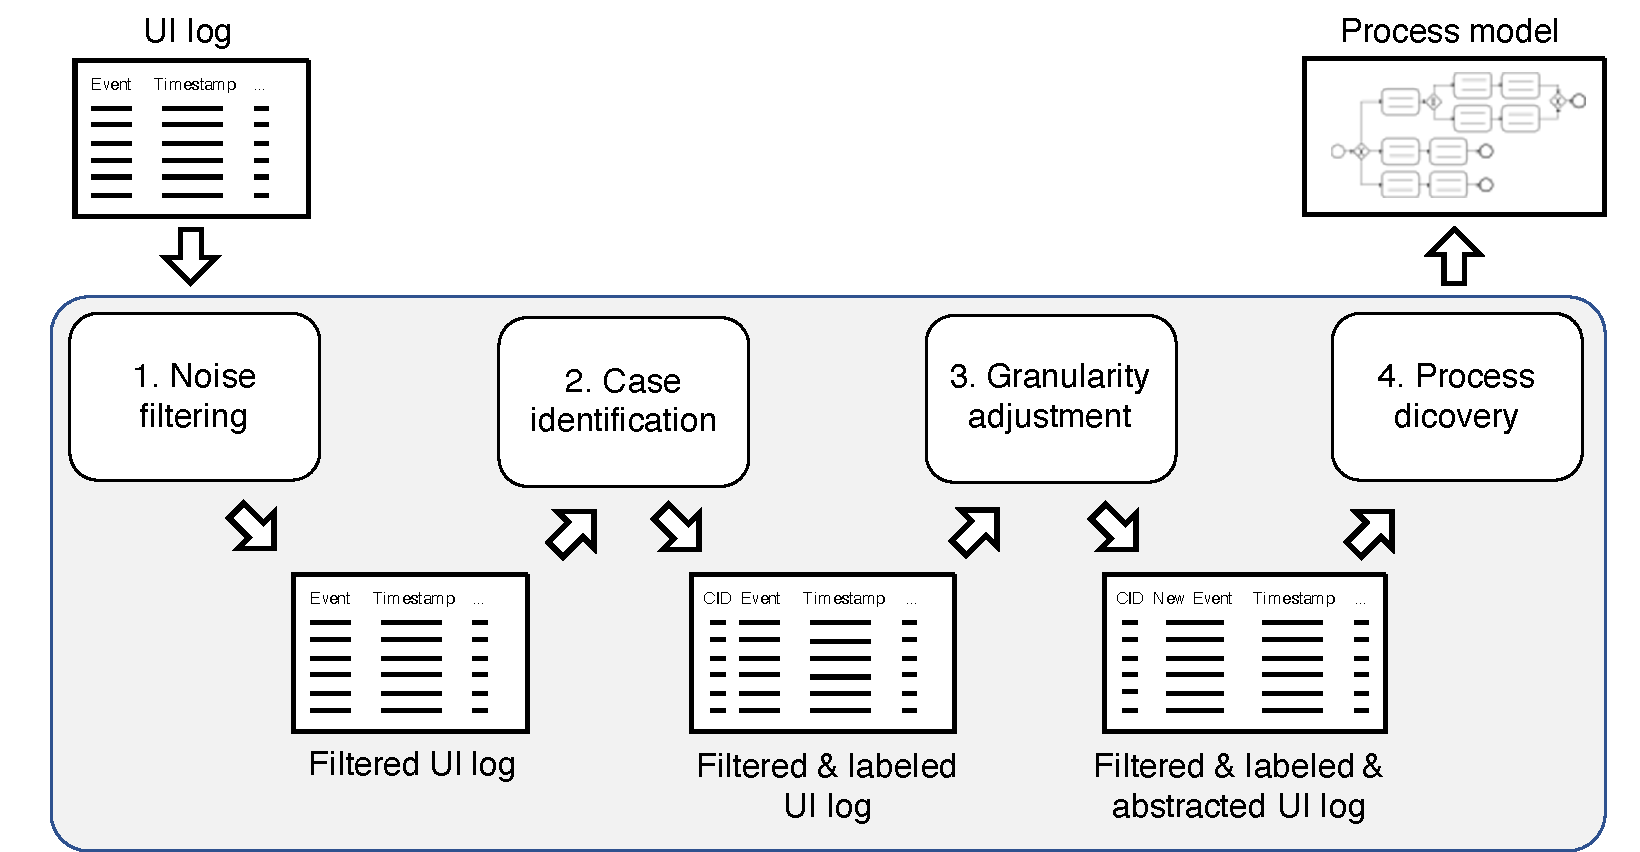
\includegraphics[width=0.9\textwidth]{figures/approach.pdf}
\caption{Overview of proposed technique}
\label{fig:approach}
\end{figure}




%The input for the technique is a set of social media posts and a set of event logs\footnote{Note that the technique does not require more than a single event log, but is simply able to handle several event logs.}. 
%The \textit{first step} of the technique is concerned with identifying and extracting weaknesses in the social media posts. This will be achieved by building on NLP tools such as dependency parsers and sentence classification techniques (see work package 1, Section \ref{sec:wp1}). The goal of the \textit{second step} is to identify the links between the identified weaknesses and the events from the event logs. To achieve this, we will  
% characterize the links between all possible weakness-event pairs by using different perspectives of similarity (see work package 2, Section \ref{sec:wp2}). Based on these link characterizations, we will then use optimization rules specified in a Markov Logic formalization to compute the most likely correspondences between weaknesses and events. The rules of the Markov Logic formalization may, for instance, specify that a weakness can only be linked to an event if the timestamp of the associated social media post indicates that the event occurred before the post was created. The definition of appropriate rules will be one of the key tasks of this project (see work package 3, Section \ref{sec:wp3}). The \textit{third step} is concerned with clustering and ranking the weaknesses. The purpose of clustering weaknesses is to recognize whether several weaknesses that are linked to a single event relate to the same \textit{weakness class}. For example, several customers may complain about waiting too long before receiving a voucher. Therefore, we would consider \textit{voucher waiting time} as a weakness class. The purpose of then ranking these weakness classes is to provide an indication of where to start with the improvement initiative. The idea is that highly ranked weakness classes are more frequent and more severe than lower ranked weakness classes. After clustering and ranking, we, therefore, can generate a weakness report that can serve as input for a process improvement initiative (see work package 4, Section \ref{sec:wp4}). 
 
%We will approach the \textit{second goal} of the project by implementing the automated technique defined in work packages 1 through 4. Moreover, we will systematically evaluate the implemented technique by applying it to different real-world data sets. While social media posts are publicly available and can be efficiently obtained via APIs\footnote{See e.g. https://developer.twitter.com/en/docs.}, event log data is harder to obtain. However, there are a number of relevant event logs that are publicly available and that we plan to use as a starting point:
%\begin{itemize}
%\item \textbf{BPI Challenge 2016}: This event log  originates from the International Business Process Intelligence Challenge from the year 2016. It contains events from the Dutch Employee Insurance Agency (UVW), which handles employee insurances and provides labor market-related services in the Netherlands. This log is well-suited for the purposes of this project because it is customer-oriented and contains text data (similar to social media posts) about customer complaints in English.
%\item \textbf{BPI Challenge 2019}: This event log originates from the International Business Process Intelligence Challenge from the year 2019. It contains (English) events from the purchase order handling process of AkzoNobel, a large multinational company with over 50 subsidiaries in the area of coatings and paints. While this log well-suited for the purposes of this project because it is customer-oriented, it does not come with textual resources created by customers. However, we will obtain relevant data from Twitter and, in this way, manually complement the log. 
%\end{itemize} 

%The implementation of the proposed technique will be conducted in Python and based on the PM4Py process mining framework\footnote{https://pm4py.fit.fraunhofer.de/} (work package 5, Section \ref{sec:wp5}). By manually creating gold standards for our evaluation data sets, we will test our technique with respect to its extraction, alignment, and clustering capabilities. We will use the evaluation results both during the project for improving our technique and at the end of the project in the context of a summative evaluation (work package 6, Section \ref{sec:wp6}). In the following, we describe the work packages in detail. Note that we provide the estimated duration of each work package in project months (PM) in the title of each work package. 

\subsection{Work programme including proposed research methods}

%We have divided the work into six work packages presented in the subsections below. In the last subsection, we give an overview on the complete project together with a time line that shows the order in which we will work on the different topics.

\subsubsection{Work package 1: Data collection and preparation  (X PM)}
\label{sec:wp1}


\subsubsection{Work package 2:  Noise removal (X PM)}
\label{sec:wp2}

As outlined in \autoref{sec:startingpoint}, UI logs often contain events that do not relate to the business process under investigation, which can include events related to private activities (e.g., checking Facebook) or to non-related business activities (e.g., filing a reimbursement form of a business trip).
Given that process mining techniques assume that the events in a log relate to a single process, these irrelevant events, also referred to as \emph{noise}, need to be identified and removed from a UI log.

While various noise detection techniques already exist (cf., \autoref{sec:stateoftheart}), these  inherently approach noise detection from a different angle. Particularly, they aim to detect process behavior that stands out in terms of frequency (such as rare occurrence of an order being accepted before it is created), i.e., they try to \emph{detect events that are behavioral anomalies}, e.g., caused by recording errors.
Instead, when dealing with UI logs, we need to \emph{detect events that do not relate to the process at hand}. 

\mypar{Semantic noise detection}
Therefore, to approach this task, we propose to develop a semantic noise detection approach tailored to the specifics of UI logs, which aims to classify events as \emph{process relevant} or not. 
To achieve this, we transform the textual payload of each event into a feature vector.
For this, we can simply concatenate all textual attribute values, followed by basic pre-processing steps such as stop-word removal and lemmatization. Yet, we will also develop a process-specific feature extraction technique, which aims to identify those textual attributes that have a specific role relevant to a process, such as involved \emph{business objects} (e.g., an \emph{order} or a \emph{ticket}), actions applied to these objects (e.g., \emph{create} or \emph{accept}), and involved people or systems. To achieve this, we aim to combine and adapt existing techniques for the recognition of semantic process components in textual attributes~\cite{rebmann2021extracting} and the extraction of actions from free-text log attributes~\cite{gupta2020analyzing}.

Once events are transformed in such feature vectors, noise identification can be approached as either a single-class or a two-class classification problem, using state-of-the-art text classifiers such as BERT~\cite{Devlin2019}. The former involves training a classifier that recognizes which events are related to a specific process, e.g., by assuming that the majority of events in a UI log are related to that. While such an approach thus would not require any user input, the classification accuracy may be improved in a two-class setting, where users explicitly label some events as process relevant and irrelevant, so that few-shot learning techniques can be employed~\cite{yu2018diverse}.
While such classifiers can be employed with just a UI log as input, we will also incorporate mechanisms that allow user to provide additional domain-specific information about the process at hand, such as textual documentation or (high-level) process models, which can help the classifier to better distinguish process relevant from irrelevant events.

\mypar{Work package outcome}
The outcome of this work package is a classification approach that identifies irrelevant events in a UI log. The approach will be applicable without requiring any additional user input, though users may improve the approach's accuracy through manual labeling of events, as well as by supplying further process-specific artifacts (e.g., a process model) as input.
%This work package focuses on the classification of events in a UI log and the subsequent identification and  removal of irrelevant, i.e., noisy, ones.
%
%\mypar{Event classification}
%\todo{maybe this should be a separate work package? since it also comes with some particular challenges}
%Process mining techniques assume that each event in a log is associated with a particular event class, denoting the action to which the event corresponds~\cite{van2016data}, such as ``\emph{accept order}'' or ``\emph{pay invoice amount}''.
%However, such event classes are not readily available for UI logs. Rather, as shown in  \autoref{fig:example}, events are characterized by various attributes in their payload, which jointly indicate the type of step that is being performed. 
%%For instance, in the form of  the respective application (e.g., Outlook or Chrome) and other details, such as the specific element in the application (e.g., an e-mail or a particular window) and relevant values (e.g., the subject and content of an e-mail). 
%To transform a UI log into an event log that can be employed in process mining, 
%each event needs to be assigned a specific event class based on its payload attributes, which may differ across UI logs or even for different events in the same log. For example, we strive to recognize that certain e-mails refer to the \emph{creation of an order}, whereas other e-mails may correspond to the \emph{handling of an order}. Though these are  two distinct process steps, they nonetheless involve the same application (e.g., Outlook), element (a particular e-mail), and likely the same e-mail subject. Therefore, we need to recognize that the content of the e-mail, as well as its position in a log, relative to related events, determine the event class in this case.
%
%To perform this classification, we recognize that process steps  can be primarily characterized by a combination of a business object (e.g., an \emph{order} or a \emph{ticket}) and an action applied to the object (e.g., \emph{create} or \emph{handle})~\cite{ref}. 
%To recognize these two components in UI events, we aim to combine and adapt existing techniques for the recognition of semantic process components in textual attributes~\cite{rebmann} and the extraction of actions from free-text log attributes~\cite{gupta2020analyzing}. Afterwards the identified event classes can be refined or grouped by employing techniques for the recognition of duplicate~\cite{ref} or polluted event labels~\cite{ref}.
%
% 
% 
% \mypar{Noise removal}
%
%\begin{itemize}
%\item Would be great to go beyond rules here. 
%\item Type 1: Repetitive actions, actions without any effect, and actions that overwrite past actions. 
%\item Type 2: Non-business related stuff: Facebook etc. However, also irrelevant e-mails.
%\item Can we use some sort of semantic angle here? Not sure whether we can determine the domain of a process and just kill anything that is unrelated or so. 
%\end{itemize}
%
%\mypar{Outcome}

\subsubsection{Work package 3: Case identification (X PM)}
\label{sec:wp3}

Once the irrelevant events have been filtered out of a UI log, we next need to recognize which events belong to the same process instance, e.g., to the same customer order or service ticket, a task referred to as \emph{case identification}.

Existing techniques that address this task in general process mining settings primarily base the identification on co-occurrence statistics, which reveal behavioral regulations in an event log (cf., \autoref{sec:stateoftheart}). While such techniques work well for relatively structured settings, their performance deteriorates for event logs stemming from more flexible environments in which the execution of several cases overlaps, such as e.g., seen in the example of \autoref{fig:example}, the first three events each start a new process instance, by initiating three different orders in a batch-like manner.

\mypar{Instance-based event matching}
Recognizing this challenge, this work package sets out to develop a new approach for case identification, tailored to the specifics of UI logs, by building on semantic matching technology.
Specifically, to determine the likelihood that events belong to the same case from a semantic viewpoint, e.g., because both refer to a same order ID or mention the same customer name, we frame the comparison of the events as an \emph{instance-based schema matching} task. For this, we recognize that events stemming from a particular application can be represented as instance in a particular schema (characterized by their payload attributes), enabling the application of existing matching techniques (cf., \cite{somerefs}).

\mypar{Optimization} Having obtained similarity scores between individual events, these scores can then be used together with behavioral regularities identified by existing techniques~\cite{ref}, and cardinality constraints (e.g., each event belongs to exactly or at most one case), to establish an optimization problem, specifically using Markov logic formulation. By solving this problem, we will obtain an event grouping that maximizes the semantic similarity and respects the identified behavioral regularities.

\mypar{Outcome}
The outcome of this work package is a case identification approach that assign case identifiers to the events in a (filtered) UI log, such that the new log encompasses a number of cases, each corresponding to a sequence of events related to the same process instance.




%\begin{itemize}
%\item It would be great to have some interesting angle here; maybe based on optimization. 
%\item We probably first need to detect start and end of a case 
%\item I was thinking of some semantic perspective that helps to identify which events belong together, e.g. based on the data that are used. 
%\item Overlapping cases (batching) might impede the use of co-occurrence-based statistics
%\end{itemize}

\subsubsection{Work package 4: Event abstraction (X PM)}
\label{sec:wp4}

\begin{itemize}
\item In the end, similar to WP3: we need to detect what belongs together. Not even sure about the order to be honest. 
\item You did something in that area, didnt you?
\end{itemize}

\subsubsection{Work package 5: Event labeling (X PM)}
\label{sec:wp5}

\begin{itemize}
\item We should bring some semantic perspective in. Maybe from text summarization. 
\end{itemize}

\subsubsection{Work package 6: Discovery (X PM)}
\label{sec:wp6}

\subsubsection{Work package 7: Summative Evaluation (X PM)}
\label{sec:wp7}


\subsubsection{Overview on the work plan}

%As explained above, the project consists of six work packages. Naturally, there are interdependencies among these work packages. Figure \ref{fig:workplan} shows a simplified work plan that mostly abstracts from parallel and overlapping work. The only work package that is shown to be conducted in parallel is work package 5 (i.e., the implementation),  which is spread over a total of 24 months. It is important to highlight that the transitions between two packages won't be as strict as depicted. We are aware of the various interdependencies  (e.g. between work packages 2 and 3) and will take them into account appropriately.  
%%There are, for instance, interdependencies between work package 2 and 3. If the similarity measures are not appropriate, this cannot be compensated by ``smart" modeling. We are fully aware of these interdependencies and will take them into account appropriately. 
%However, the rather abstract view on the work plan shown in Figure \ref{fig:workplan} highlights our general idea of having two main iterations:
%\begin{itemize}
%\item The first iteration ends after 21 month. At the end of this iteration, there will be a first implemented prototype available, which we tested in the context of a first comprehensive evaluation. The outcome of this evaluation will provide valuable insights into the strengths and weaknesses of our technique and, therefore, determine which components need to be improved. 
%\item The second iteration is slightly shorter and will be mainly used to address identified weaknesses and improve the performance of the technique. What is more, it contains work package 5, which will be used to group and rank the results from work package 4. Finally, we will perform a summative evaluation and compare our approach to established process mining techniques. 
%\end{itemize} 
%
%\begin{figure}[h!]
%\includegraphics[width=\textwidth]{Figures/timeline.pdf}
%\caption{Work plan}
%\label{fig:workplan}
%\end{figure}
%
%Note that the work plan shown above allocates a total of 42 project months to 3 years. As explained in Section \ref{sec:staff}, we intend to hire a PhD student for 3 years, which means that remaining 6 project months will be covered by the principal investigator of this project. 